\chapter{Introduction}
\paragraph*{}
Ce projet de machine learning nous a été proposé dans le cadre du cours de Gestion et valorisation de projet en Machine Learning (GML), donné au cours du cinquième semestre du cursus de Bachelor en Informatique et système de communication orienté ingénierie des données à la HEIG-VD. Le but de ce travail est de nous faire découvrir la gestion et organisation impliquée par un travail de machine learning, autant au niveau de la recherche technologique qu'au niveau de l'organisation d'équipe, notamment au niveau de la distribution de tâches, gestion d'équipe et de délais. \newline

Le projet décrit ici est un projet existant ayant déjà été réalisé plusieurs fois par le professeur et de précédents étudiant.e.s : l'étude de crapauducs. Un crapauduc est un “petit conduit sous une route, permettant le passage protégé des batraciens” - selon Le Robert. En 2017, dix-huit crapauducs ont étés construits le long de la route d'Aubonne à Gimel - canton de Vaud - afin de permettre aux grenouilles, crapauds et tritons de traverser la route des bois à l'étang en toute sécurité, L'image \ref{fig:Un des 18 crapauducs installés pour l'étude} en montre un.. \newline

À l'intérieur de ces crapauducs ont été installée une caméra équipée d'un capteur, qui implique la prise d'une petite série de photos (\textit{Figure 1.2}) lors de la détection de mouvement, ainsi qu'une planche afin de faciliter la distinction des objets du sol. Comptant moins de caméras que de crapauducs, les caméras n'étaient pas rattachée à un crapauduc et comptent donc des images prises depuis différents crapauducs.\newline

\begin{figure}[!htb]
    \centering
    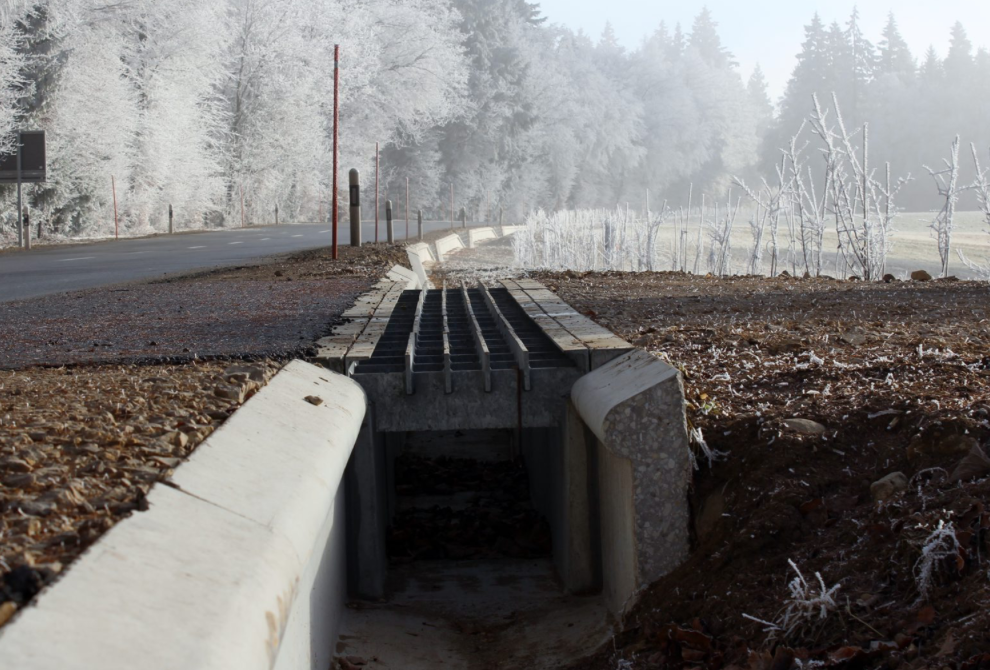
\includegraphics[width=200px]{images/introduction_crapauduc_exterieur.png}
    \caption{Un des 18 crapauducs installés pour l'étude}
    \label{fig:Un des 18 crapauducs installés pour l'étude}
\end{figure}

\newpage

\begin{figure}[!htb]
    \centering
    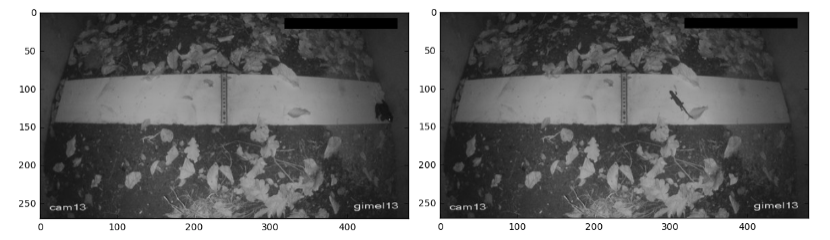
\includegraphics[width=300px]{images/introduction_crapauduc_exemple_prise_camera.png}
    \caption{Exemples des images d'amphibiens prises par les cameras}
    \label{fig:Exemples des images d'amphibiens prises par les cameras}
\end{figure}

Au terme de la première année d'utilisation, ces voies ont été empruntées par plus de 6'000 crapauds, grenouilles et tritons confondus. Ce comptage a été effectué par des chercheurs, qui ont du regarder les images prises par les caméras et compter les animaux "à la main". Le projet Crapauduc vise ainsi à utiliser l'apprentissage automatique (Machine Learning) pour automatiser le comptage des batraciens. \newline

Notre objectif pour ce projet est donc de détecter la présence ou non de grenouille/crapaud et tritons (en considérant les grenouilles et crapauds comme une seule et même catégorie) en utilisant l'apprentissage automatique, ce afin de déterminer si la constructions de ces crapauducs est efficace. Pour se faire, nous avons les prises des caméras du 23 février 2017 au 20 avril de la même année, totalisant près de 1 million d'images, dont on connaît pour chacune la caméra dont elle provient ainsi que le moment où la photo a été prise (date, heure, minute et seconde).\newline

Enfin, le professeur Satizabal Mejia Hector Fabio nous a également mis à disposition sa labelisation pour certaines images, des bounding box pour certaines également, ainsi que les données météos enregistrées durant cette période (notamment la température, le vent, la précipitation et l'humidité).


